The swimlane diagram shown in Figure ~\ref{fig:the_process} on page
~\pageref{fig:the_process} has three classes of swimlane:

\begin{itemize}

   \item Development Artefacts - these are items that are either consumed or generated by
         a process activity. This will include the solution to the problem, together with
         the design and test artefacts produced during the creation of the solution.

   \item Development Activites - these are the tasks to be performed to address the
         development goals of the project. The development activities are split across
         swimlanes representing different Team Member rolls within the project:

         \begin{itemize}
            \item Requirements Engineer
            \item Development Engineer
            \item Test Engineer
         \end{itemize}

    The development steps in the swimlane diagram are part of the applied techniques
    listed below :

         \begin{itemize}
            \item \reveal\ - Development Context Diagram; Elicit Requirements; Boundary
            identification; Develop Project Data Model; Develop Domain, Specification,
            Requirements and Satisfaction Argument.
            \item \informed\ - Develop \informed\ Architecture; Apportion requirements to
            Architectural components; Develop UML Diagrams (Optional).
            \item SPARK2014 code development - Refine Specification statements based upon
            architectural structure; Develop Code, Statically Analyse Code; Develop
            High-Level Test Conditions; Develop AUnit High-Level Test Cases; Develop Module
            Test Conditions; Develop Module Tests and relevant stubs; Exceute Tests.
         \end{itemize}

    Prior to the execution of the project two activities have been applied, these are: Process
    Definition and Tool Selection.  Process design is applied to all \altran\ projects, and is
    tailored to select Procedures and Processes from a library of techniques, and is intended
    to produce an optimal mechanism to deliver the solution.

    \item Infrastructure - identifies the tools used in the solution of the problem.
\end{itemize}

\begin{sidewaysfigure}[p]
    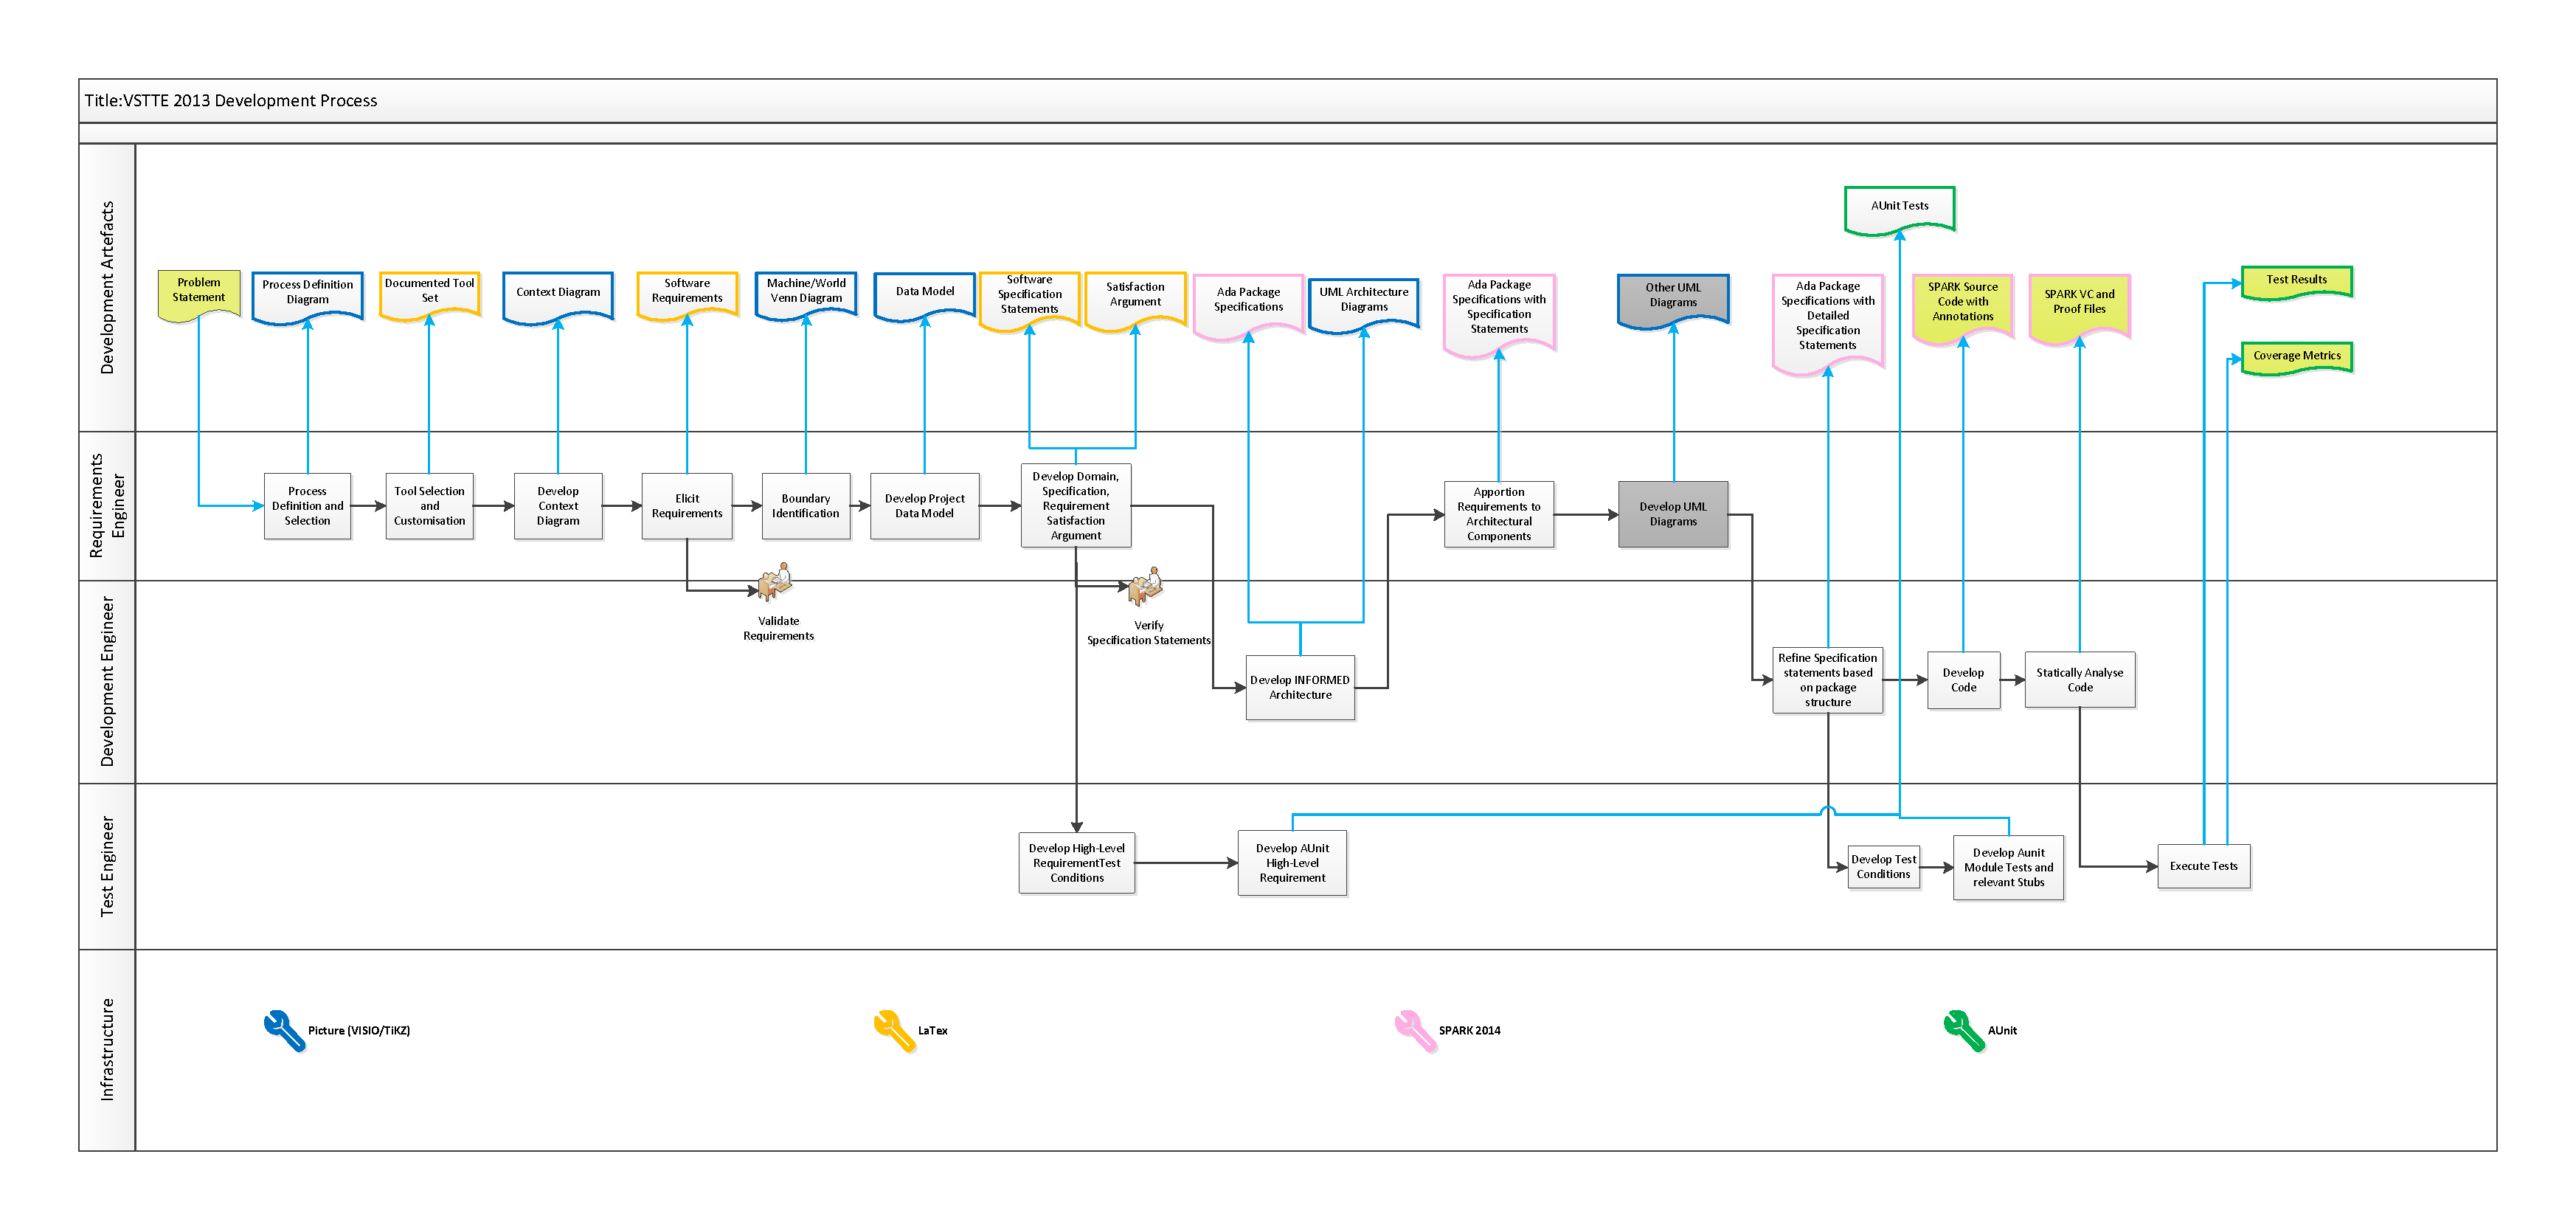
\includegraphics[width=\textwidth]{SwimLaneProcessDiagram.pdf}
    \caption{Our process}
    \label{fig:the_process}
\end{sidewaysfigure}

\clearpage

\section{\reveal\ Overview}
\label{REVEALOverview}
Software Engineering is concerned with the controlled and correct
development of Systems (Machines) that impact upon the environment in
which they are deployed (World). Where the objective of the deployment
of a Machine is to improve the World.

The purpose of Requirements Engineering is to take a set of
Stakeholder Requirements and arrive at a complete, correct and usable
set of System Specification Statements for the system under
development. Within \reveal\ the application of the
process is also intended to have a wider objective of adding benefits
to the project Stakeholders through learning, negotiation and the
development of trust between all parties involved in the production of
the system.

\reveal\ is Altrans' systematic method for the
elicitation, specification and management of System
Requirements. Through its application we clearly identify three key
artefacts:

\begin{itemize}
\item Requirements (R) which are statements about things in the World
  that we want the System to make true.

\item Specification Statements (S) describe the Systems external
  behaviour.
  \begin{itemize}
  \item Specifications include only shared phenomena in the interface
    between the World and the System being developed.
  \item Specifications can only constrain shared phenomena that the
    System can control.
  \end{itemize}

\item Domain Statements (D) which are knowledge about the World, that
  is generally assumed and not normally documented, but must hold if
  the Specification Statements are to fully satisfy the System
  Requirements.
\end{itemize}

Once this information has been gathered, a Satisfaction Argument is
constructed to show that all the Stakeholder Requirements have been
addressed through the System Specification and Domain Statements. (As
Verification and Validation progresses, V\&V Plans and summary results
can also inform the satisfaction argument, although this may not be
done for the competition.)

The \reveal\ process is far more extensive than that
described above including detailed processes for:
\begin{itemize}
\item Stakeholder Identification,
\item Knowledge Elicitation,
\item Requirement Verification and Validation,
\item Conflict Management and Resolution,
\item Requirements Maintenance and Management.
\end{itemize}

More information on the \reveal\ method can be found on
\url{http://intelligent-systems.altran.com/technologies/systems-engineering/revealtm.html}.

Since by its nature the VSTTE 2013 competition has a very short
timescale, and the Requirements are provided by the competition
organisers it is not expected that there would be time to apply a full
\reveal\ process, however the benefits of Requirements
capture, expression, satisfaction arguments and traceability can be
shown by their application in this context.



\section{\informed\ Overview}
\label{INFORMEDOverview}
\informed\ is the Altran method for the construction of high-quality
software at a low-cost, it uses elements of both object oriented (OOD)
and functional design. OOD is used to establish the architecture of
the system and the elements of system state it contains. The result is
an annotated framework of SPARK packages, constructing an architecture
that is modifiable and maintainable, which is capable of being
analysed at an early stage using the Examiner.

Altrans' analysis of many software designs has identified that there
are 3 key building blocks that are used repeatedly to build an
application. These building blocks are:

\begin{itemize}
\item A Main Program, that is the top level, entry point controlling
  the behaviour a system or sub-system.
\item Variable Packages, which are SPARK packages containing
  persistent "state", and are equivalent to what is commonly called an
  object.
\item Type Packages, which define the name of a type, and the
  operations taht it supports.
\end{itemize}

\noindent
In addition to these packages, \informed\ also includes two other
types of packages:

\begin{itemize}
\item Utility Packages, which provide shared functionality. The need
  for utility packages arises when an operation is required which
  affects or uses more than one variable of type package.
\item Boundary Variable Packages, which are particular kinds of
  variable package which provides interfaces between the software
  functionality described by the \informed\ design and elements
  outside it with which it must communicate. Unlike other variable
  packages the variable within the package is a place holder
  representing the stream of data arriving from, or being sent to, the
  outside world rather than simply an abstract name for the internal
  state of the package.
\end{itemize}

\noindent
The \informed\ method consists of 6 steps, and these are:

\begin{enumerate}
\item Identification of the System boundary, inputs and outputs.
\item Identification of the SPARK boundary.
\item Identification and localization of the system state.
\item Handling initalization of state.
\item Handling secondary requirements.
\item Implementing the internal behaviour of components.
\end{enumerate}

\noindent
The output of the \informed\ process is represented a collection of
design diagrams and a collection of well defined SPARK
specifications. A summary of the \informed\ graphical elements and
example representations are documented in Annex A of this document to
aid the reader in the understanding of the architectural design.

As the VSTTE 2013 competition has a very short timescale, it is not
expected that there is enough time to fully apply the \informed\
process, however the benefits of the benifits of the modelling
approach and the translation in SPARK Package Specifications can be
shown in this project.

